\begin{pastexam}[label={px:ncu-115-dsa-13}]{中央資工所 115 學年度 第 13 題}
（複選；每題 5 分，全對才給分，答錯倒扣 1 分）

Given a weighted undirected graph G (V, E) below. Which of the following statement(s) about the
minimum spanning tree (MST) of G is (are) true?
\begin{center}
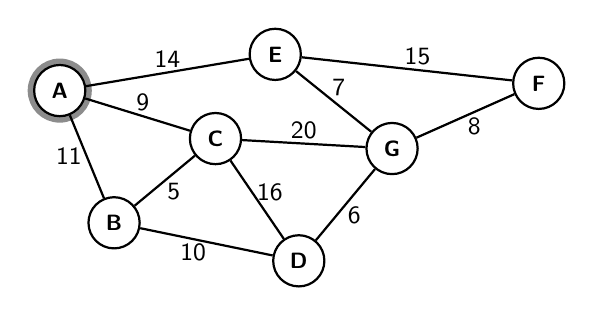
\begin{tikzpicture}[v/.style={circle,draw,thick,fill=white,minimum size=6.5mm,inner sep=0pt,font=\footnotesize\sffamily\bfseries},x=1.15cm,y=1.15cm,
  w/.style={font=\small\sffamily,inner sep=1.5pt}]
\node[circle,draw=black!45,line width=2.4pt,minimum size=7.3mm,inner sep=0pt] at (0,1.88) {};
\node[v] (A) at (0,1.88) {A};
\node[v] (E) at (2.38,2.28) {E};
\node[v] (F) at (5.29,1.96) {F};
\node[v] (C) at (1.72,1.35) {C};
\node[v] (G) at (3.67,1.24) {G};
\node[v] (B) at (0.60,0.42) {B};
\node[v] (D) at (2.64,0) {D};
\draw[thick] (A) -- node[w,above,pos=0.5] {14} (E);
\draw[thick] (A) -- node[w,above,pos=0.55] {9} (C);
\draw[thick] (A) -- node[w,left,pos=0.5] {11} (B);
\draw[thick] (E) -- node[w,above,pos=0.55] {15} (F);
\draw[thick] (E) -- node[w,above right,pos=0.45,inner sep=0.5pt] {7} (G);
\draw[thick] (C) -- node[w,above,pos=0.5] {20} (G);
\draw[thick] (C) -- node[w,below right,pos=0.5,inner sep=0.5pt] {5} (B);
\draw[thick] (C) -- node[w,right,pos=0.4] {16} (D);
\draw[thick] (B) -- node[w,below,pos=0.4] {10} (D);
\draw[thick] (D) -- node[w,below right,pos=0.5,inner sep=0.5pt] {6} (G);
\draw[thick] (G) -- node[w,below right,pos=0.5,inner sep=0.5pt] {8} (F);
\end{tikzpicture}
\end{center}
\begin{enumerate}[label=\Alph*.]
\item If the MST is constructed by Kruskal's algorithm, edge (E, G) is the 6-th edge added to
the MST.
\item If the MST is constructed by Kruskal's algorithm, the MST is a binary tree.
\item If the MST is constructed by Prim's algorithm and starting from vertex C, edge (E, G) is
the 5-th edge added to the MST.
\item If the MST is constructed by Prim's algorithm and starting from vertex D, there is an edge
connecting vertex A and vertex B.
\end{enumerate}
\end{pastexam}

\begin{pastsoln}
答案：B、C。 C 一定對；B 要看「二元樹」怎麼解讀（見下面），本書採用的解讀下也對。 A、D 錯。

\textbf{先求最小生成樹。} 十一條邊的權重都不同，由資結書定理~24.4，最小生成樹只有一
棵，不論用哪個演算法、從哪裡開始，選到的邊集合都一樣，只有\textbf{順序}會不同。 Kruskal 依權重
由小到大：

\begin{center}
\small
\begin{tabular}{rcrl}
\toprule
步 & 邊 & 權重 & 結果 \\
\midrule
1 & B--C & 5 & 選（第 1 條） \\
2 & D--G & 6 & 選（第 2 條） \\
3 & E--G & 7 & 選（第 3 條） \\
4 & F--G & 8 & 選（第 4 條） \\
5 & A--C & 9 & 選（第 5 條） \\
6 & B--D & 10 & 選（第 6 條）；$\{A, B, C\}$ 和 $\{D, E, F, G\}$ 接起來，已滿 $6$ 條 \\
\bottomrule
\end{tabular}
\end{center}

後面的 A--B（$11$）、A--E（$14$）、E--F（$15$）、C--D（$16$）、C--G（$20$）都不用看（它們的兩端
都已經連通）。 最小生成樹是 $\{BC, DG, EG, FG, AC, BD\}$，總權重 $5 + 6 + 7 + 8 + 9 + 10 = 45$。

\begin{itemize}
\item \textbf{A. 錯。} E--G 是 Kruskal 加入的第 $3$ 條邊，不是第 $6$ 條；第 $6$ 條是 B--D。
\item \textbf{B. 看解讀。} 最小生成樹是一棵沒有根的樹，各頂點的度數是 A：$1$、B：$2$、C：$2$、
D：$2$、E：$1$、F：$1$、G：$3$，形狀是一條 A--C--B--D--G 的鏈，G 再接出 E、F 兩個葉節點。
「二元樹」要先有根才談得上「每個節點最多兩個子節點」。 如果解讀成「可以選一個頂點當根，讓它
變成二元樹」：選 A 當根，A、C、B、D 各只有一個子節點，G 有 E、F 兩個子節點，是二元樹，(B)
對。 如果要求選哪個頂點當根都要是二元樹，選 G 當根時它有 D、E、F 三個子節點，(B) 錯。 本書採
前一種解讀（最大度數 $3$ 的樹，以葉節點為根就是二元樹），但這一項的敘述本身不嚴謹，作答時最好
寫出你的解讀。
\item \textbf{C. 對。} 從 C 開始執行 Prim 演算法（資結書虛擬碼~24.3），每回合取出
$\mathit{key}$ 最小的頂點：

\begin{center}
\small
\begin{tabular}{cclc}
\toprule
回合 & 取出 & 加入的邊 & 取出後改小的 $\mathit{key}$ \\
\midrule
1 & C & — & A：$9$，B：$5$，D：$16$，G：$20$ \\
2 & B & C--B（$5$），第 1 條 & D：$10$（A 的 $11$ 不比 $9$ 小） \\
3 & A & C--A（$9$），第 2 條 & E：$14$ \\
4 & D & B--D（$10$），第 3 條 & G：$6$ \\
5 & G & D--G（$6$），第 4 條 & E：$7$，F：$8$ \\
6 & E & G--E（$7$），第 5 條 & （F 的 $15$ 不比 $8$ 小） \\
7 & F & G--F（$8$），第 6 條 & \\
\bottomrule
\end{tabular}
\end{center}

E--G 是第 $5$ 條加入的邊。 這張表裡沒有平手，平手規則不影響結果。
\item \textbf{D. 錯。} 最小生成樹唯一，Prim 演算法從 D 開始選到的也是上面那六條邊，裡面沒有
A--B。 A--B 不在任何最小生成樹裡也可以直接看出來：環 A--B--C--A 的三條邊是 $11$、$5$、$9$，
A--B 是這個環上唯一最重的，由環性質（資結書定理~24.3）一定不選。
\end{itemize}
\end{pastsoln}
